% !TEX root = ../Main.tex
\subsection{Size vs Frequency}
In \cref{Fvms} we achieved the result of $f=\dfrac{1}{x^{1.4}}$ when fitting to the data. \\
The frequency for a classic membrane is proportional to the velocity of the wave divided by the radius of the membrane $\omega \propto \dfrac{v}{x}$. But for a layer of graphene the velocity of the wave is proportional to the frequency which then again is proportional to the inverse radius $v\propto\omega\propto\dfrac{1}{x}$. This means the frequency becomes proportional the the inverse radius squared $\righarrow \omega \propto \dfrac{1/x}{x}=\dfrac{1}{x^{2}}$ In the real space of our lattice these two results corresponds to $\dfrac{1}{x}$ and $\dfrac{1}{x^{2}}$ This means that our value of the exponent $n=1.4$ lies somewhere in between the frequency for a classic and a graphene memebrane. The reason for this is because of the very small membranes we have included in our data. The limit around the perimeter of the membrane is infinitely thin from a classic perspective, but for our system the limit consist of atoms which have non neglectible effects on the frequency, why we see a dependency of the radius which is in bewteen the classic and graphene models. 
% Removing the first couple of data points while adding more data point for bigger membranes might have given a result closer to the $\dfrac{1}{x^{2}}$ value as this band represents the out of plane motion, which is what we see when looking at modes. 
\subsection{Interlayer interaction}
In \cref{InterInter} we found that an $\epsilon$ corresponding to a substrate of silicon dioxide in the interlayer Lennard Jones potential, had an $10.1\%$ average frequency deviation from the idealised clamped membrane. The average deviation are showed on \cref{MFD}. Silicon dioxide turned out to be the best of the two candidates. As of such we now know that silicon dioxide is a suitable candidate as a substrate, if we were to simulate vibrational modes in a single layer membrane and then test the vibrational modes in the lab, where a substrate is needed. This is not a final result as other materials might be better suited and another research project could consist in determine the optimal theoretical $\epsilon$ value, and then find materials with such a value (or as close as).

\subsection{Comparison of findings in other works}
As mentioned in the introduction, we have seen that nanomembranes can contain localised modes on the microscale (see \cref{Motivation}\cite{Davidovikj2016}). This tendency is clearly continued on the nanoscale as we find modes with similar behavior (\cref{BIG}). Comparing these results motivates experimental tests of membranes on the nanoscale in the lab.

\subsection{Further analysis of the system}
Following the analysis which has been worked through, the next natural step would be to look at the how the energy of a single mode disperses in a situation where membrane is held at its maximum displacement for a given mode and then let go. After analysing such a situation we would follow up by expanding the model, adding another membrane to see how the coupling between them changes as distance between them is varied. The goal of this kind of analysis would be to find the distance between the membranes where there is no coupling between them.

\subsection{Perspective: Going from theory to the lab}
With the result from the analysis of the simulations, the next logical step would be to make tests in a lab to get measurements for comparison. \cref{FDC} is a proposed experiment you could make to get this data. What is going to happen is that the laser will drive a oscillation in the membranes, which in turn will increase and decrease the distance between the graphene layer and the metal conductor. Because the substrate will act as a dielectric this creates a parallel-plate capacitor, which has a capacitance $C$ that can be calculated as $C=\dfrac{\varepsilon\cdot A}{d}$ where $\varepsilon$ where is the permittivity, $A$ is the area that which the two plates share, and $d$ is the distance between the plates. As we found out in the analysis of the two layered system the frequencies needed to drive the membranes were in the terahertz spectrum and therefore a terahertz laser would be needed to drive the membrane in the experimental setup. The calculated frequencies can be seen on \cref{freqclamp,,freqval} Since the membranes effectively change the distance between the plates of the capacitor and thereby the capacitance they can be used to create an electric signal that match the analogue signal of the membrane. That is our proposal for getting data in the lab.

\begin{figure}[H]
  \centering
  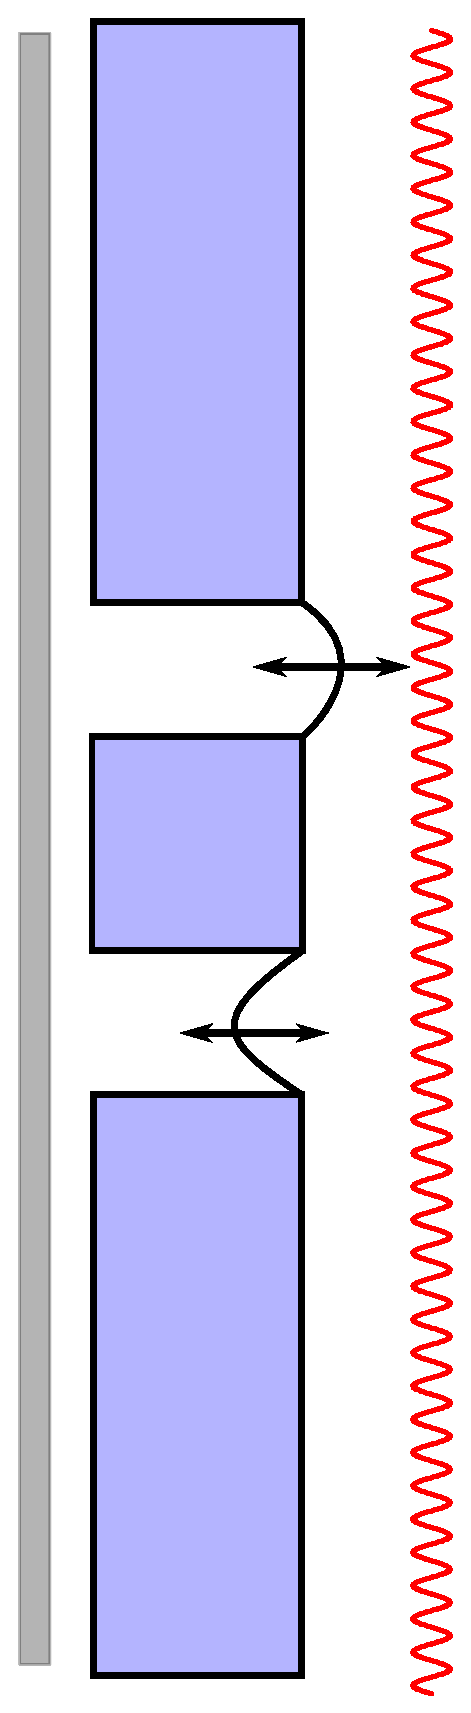
\includegraphics[width=0.3\columnwidth]{Figures/Fuck_dig_christoffer.eps}
  \caption{The setup of our proposed experiment, with the substrate (blue), the laser (red), the conductor (grey) and the membrane(black)}
  \label{FDC}
\end{figure}